\section{Introduction}
In this chapter will be presented the architecture of CPIM especially for the NoSQL service as it was before this work, then will be explained how was possible to include Kundera as persistence layer for the NoSQL service in CPIM and what problem has been faced during the process.
Furthermore in section \ref{sec:hegira} is shown how the integration with the migration system \textit{Hegira} has been introduced, what are the feature supported by this integration and which design choices has been put in place. 

\section{CPIM architecture}
To be able to expose a common interface for the multiple services supported by the library, CPIM adopts heavily the factory and singleton patterns.

\noindent The main access point of the library is the \texttt{MF} (Manager Factory) a singleton object which is responsible of reading the configuration files and exposing a set of methods that will build instances for the service factories.
The initialization is done through the first call to \texttt{MF.getFactory()} which read the configuration files and build an instance of \texttt{CloudMetadata} which will be referenced by all the other services and contains all the information stored in the configuration files.
 
\newparagraph The library is organized in several packages each of one is responsible of a particular service.
\noindent Each service exposes a factory class which is invoked through the \texttt{MF} factory, the service factory maintains a singleton instance of the provider-specific service implementation which is built at the first call based on the configuration available inside the singleton instance of \texttt{CloudMetadata}.
The result of this process is that with the same method call, based on the configuration file, is instantiated one service implementation or another.

\subsection{NoSQL service}
Before this work CPIM library supports NoSQL interaction through Java Persistence API.
The interoperability with the supported clouds is made possible thanks to the previously described factory pattern, a complete class diagram for this service can be seen in the figure \ref{fig:cpim-nosql}.

\begin{figure}[tbh]
  \centering
  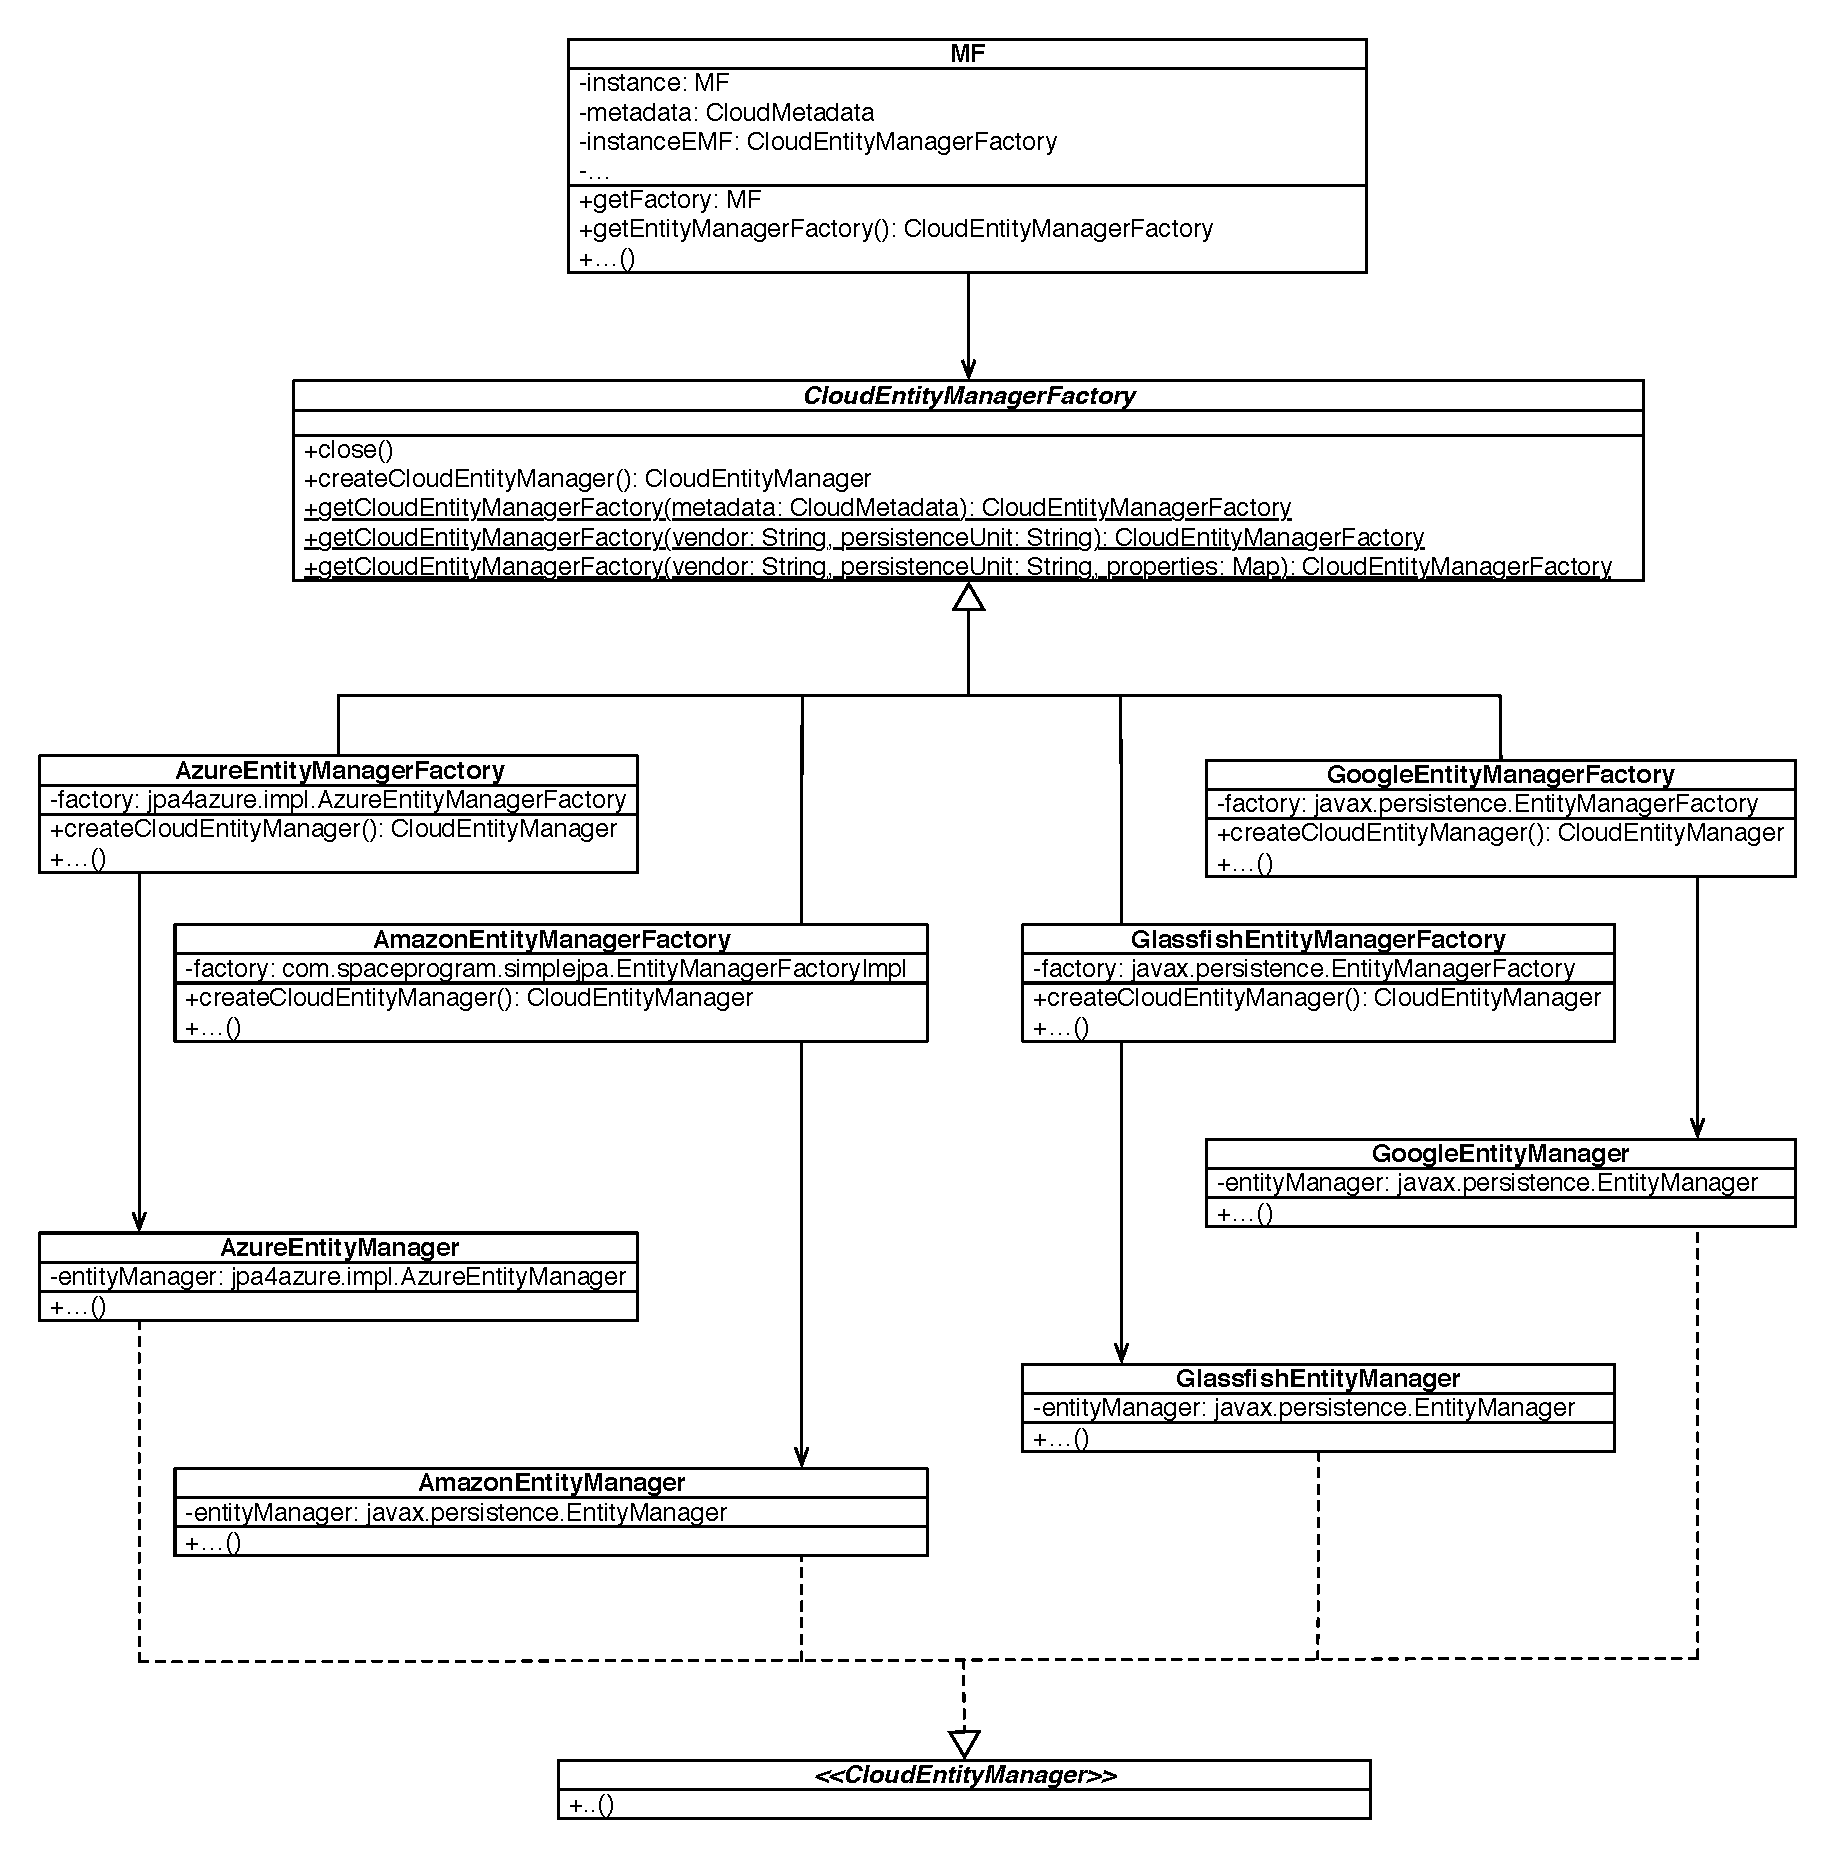
\includegraphics[width=14cm]{images/cpim_nosql_old}
  \caption{NoSQL service architecture}
  \label{fig:cpim-nosql}
\end{figure}

\noindent To use the service, the first step is instantiate a \texttt{CloudEntityManagerFactory} and, depending on the configuration file, this factory instantiate the vendor specific factory. For example in case that Google is the chosen vendor, the instantiated factory will be \texttt{GoogleEntityManagerFactory}. 
Each provider-specific \texttt{EntityManagerFactory} is responsible of instantiating an \texttt{EntityManager} which is the gateway to the underlying database. All the vendor-specific \texttt{EntityManager}(s) implement the common \texttt{CloudEntityManager} interface to achieve uniformity in methods and behavior.
The various implementation of the \texttt{CloudEntityManager} delegates every method call to the vendor-specific persistence provider. 

\newparagraph JPA is not a default language for NoSQL (as described in chapter \ref{chapter:sota}) but, due to its wide usage among Java developers, several JPA implementation has been build upon various NoSQL databases both developed by the vendor of the NoSQL storage or by the community.
This means that to support the NoSQL service through the JPA interface, an implementation of the JPA interface must be found. There are so three different persistence providers, one for each cloud provider:
\begin{itemize}
\item for \textit{Google Datastore} its used an official JPA implementation, available inside the SDK
\item for \textit{Amazon SimpleDB} its used \textbf{SimpleJPA}, a third-party implementation of the JPA interface
\item for \textit{Azure Tables} its used \textbf{jpa4azure}, a third-party implementation of the JPA interface
\end{itemize}

\noindent There are couple of things to notice: Amazon SimpleDB has been deprecated in favor of DynamoDB and \textit{jpa4azure} is not being maintained anymore, therefore CPIM needs to be updated in order to get rid of those outdated software.

\section{Kundera integration}
To solve this problems and reduce the number of software on which the CPIM rely on to provide the NoSQL service, the proposed solution  to modify the current CPIM architecture with a unique persistence provider that has been identified in Kundera.

\newparagraph The proposed solution is resumed in the architecture of figure \ref{fig:cpim-kundera} in which the benefit of having a single JPA provider are clearly visible. The architecture is slightly less articulated and no check on the selected provider is needed since this is handled by Kundera while reading the \texttt{persistence.xml} file in which the user will define what datastore is interested in.
Another benefit of this architecture is that the choice of the NoSQL technology is no more bound to the vendor specified in the CPIM configuration file, is in fact possible deploy the application in one of the supported PaaS provider and choose as NoSQL solution of another one which will be addressed remotely, simply by configuring the \texttt{persistence.xml}, moreover it's possible exploiting the Kundera polyglot persistency, to persist part of the data in a database and another part in another one defining the persistence units properly.

\begin{figure}[tbh]
  \centering
  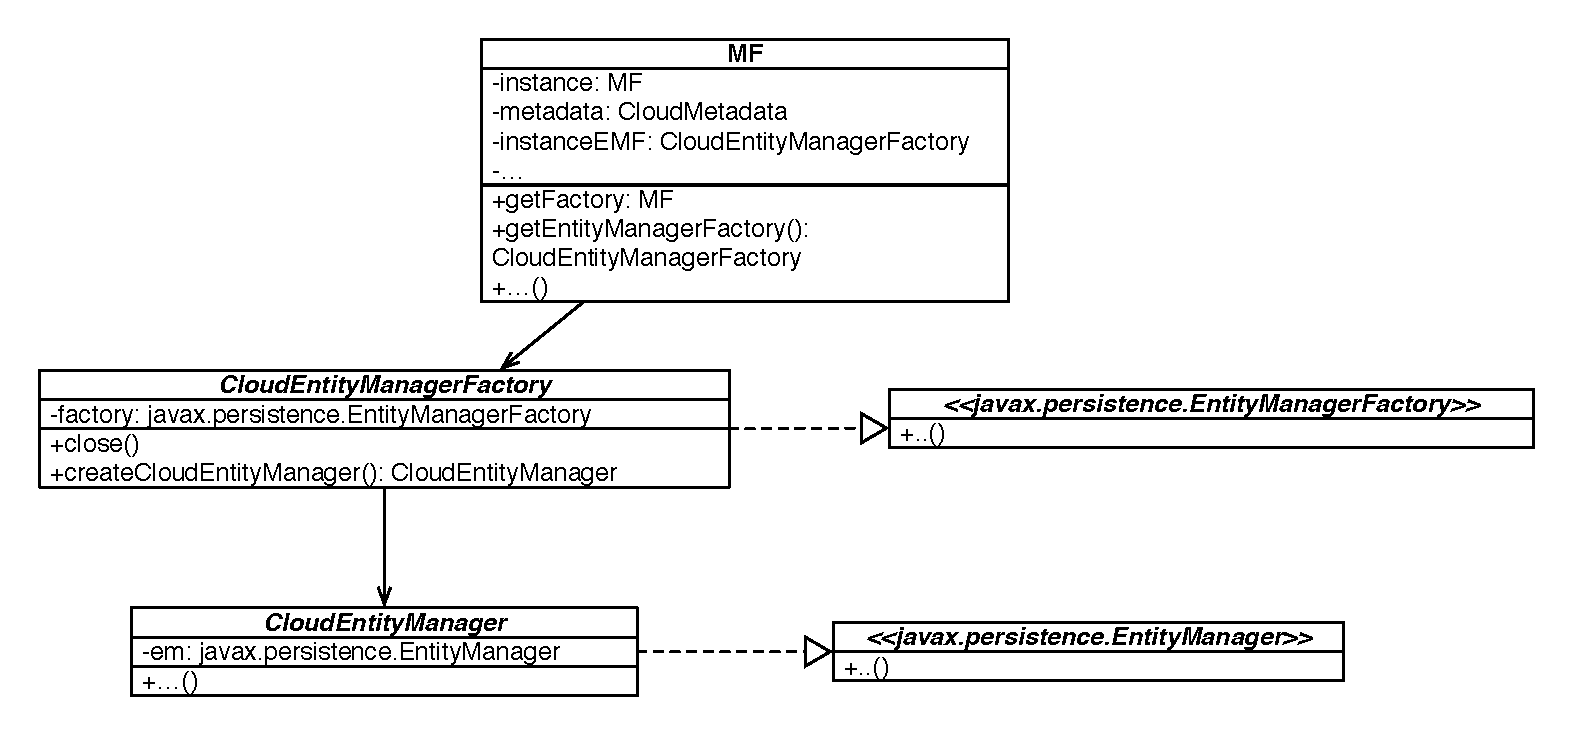
\includegraphics[width=14cm]{images/cpim_nosql_kundera}
  \caption{The modified NoSQL service architecture}
  \label{fig:cpim-kundera}
\end{figure}

\subsection{Problems encountered}
Kundera provides an uniform access through the JPA interface independently from the provider, which is somehow defined in the \textit{persistence.xml} through the Kundera client selection. For this reasons all the old libraries that provides a JPA implementation for a specific provider can be removed from the CPIM. 
This tentative in cleaning the dependency of CPIM caused two main problems:
\begin{enumerate}
\item \textit{jpa4azure} turns out to be used also for Queue and Blob service of Windows Azure
\item Kundera seems to have problem when multiple persistence provider are found in the classpath and has not be found a way to force the selection of Kundera as persistence provider (besides specifying it in the \textit{persistence.xml} file)
\end{enumerate} 

\noindent To solve the first problem, the code of the extended version of\textit{jpa4azure} has been inspected since it was extended to support some missing functionalities of the JPA interface, the library contains two main packages:
\begin{itemize}
\item \texttt{jpa4azure}, which contains the code that implement the JPA
\item \texttt{com.windowsazure.samples}, which contains the code do ease the communication with the Azure services
\end{itemize}
The \texttt{jpa4azure} package has been removed and the library rebuild since the other package is the one used in the Blob and Queue service. Its possible to completely remove \texttt{jpa4azure} but is necessary to rewrite also the CPIM Blob storage service for Azure using the Azure SDK.

\newparagraph CPIM shows more errors in the code in the Queue service and after some investigations, turns out that when \textit{jpa4azure} was extended the class \texttt{AzureQueueManagerFactory} and other were introduced.
The problem was that \texttt{AzureQueueManagerFactory} use the JPA interface to communicate with the Queue service so removing the support to JPA interface has leaded to lose the support to Azure Queue service.
One possible solution to this would be rewrite the CPIM Queue services for Azure using Azure SDK.

\section{Hegira integration}
\label{sec:hegira}
To support data synchronization and migration, the NoSQL service was further modified to integrate with \textbf{Hegira} \cite{thesis:marco}.

\subsection{Migration Manager}

\section{Intercept user operation}
The first operation that needs to be analyzed is where is possible to intercept user operation is a way that is completely transparent to the user.
The operation that we want to intercept are the insert, update and delete operation cause those are the operation that alter the structure of the data and thus are the one that needs to be processed by the migration system.

\subsection{Intercepting CRUD operations}
\subsection{Intercepting queries}
A first look at the JPQL specification \cite{book:projpa2} revealed that JPQL does not support \textit{INSERT} statements and so the only way user have to persist entities is through \texttt{EntityManager.persist(Object entity)} that is one of the case described in the previous section. The remaining case (\textit{UPDATE} and \textit{DELETE}) must be intercepted in two different situations:
\begin{enumerate}
\item queries generated through \texttt{EntityManager}
\item named queries defined as named queries 
\end{enumerate}

\noindent JPA interface provides several ways to build and execute queries all available by calling the proper methods defined in the \texttt{EntityManager} interface: \texttt{createQuery}, \texttt{createNamedQuery} and \texttt{createNativeQuery}
Native queries are clearly not supported by Kundera and thus from the migration system clearly because there not so many storage that provides a SQL-like language to specify queries.
The remaining two kind of methods to create queries are slightly different to handle.

\subsubsection{Queries through EntityManager}

\subsubsection{Named Queries}

\section{Build statements from user operations}
\subsection{Build statements from objects}
\subsubsection{Contacting the synchronization service}
\subsubsection{Handling the sequence numbers}
\subsection{Build statements from JPQL queries}
\subsection{Sending statements to Hegira}

\section{Interoperability of stored data}
The Kundera client developed and described in chapter \ref{chap:kundera} was developed to be 

\section{Summary}
In this chapter has been rapidly described the CPIM structure and the architecture of the NoSQL service before this work. Then has been described how was possible to integrate Kundera as unique persistence provider in the NoSQL service and the problem encountered in the process.

\noindent From section \ref{sec:hegira} has been described the general interaction we wanted to build to make CPIM and Hegira communicate and was then introduced and described the architecture and the design choices operated in order to develop such interaction. 